\chapter{Preliminaries}
\setcounter{page}{1}
\pagenumbering{arabic}

\section{Basic definitions and results}
\begin{definition}
An \textit{abelian field} is a finite Galois extension of $\Q$ with an abelian Galois group. 
\end{definition}

\begin{theorem}[Kronecker-Weber]
Every abelian field is a subfield of some cyclotomic field.
\end{theorem}
\begin{proof}
See \citep{washington1997}, page 321.
%\citep{washington1982}, page 319.
\end{proof}

\begin{definition}
Let $k$ be an abelian field. The least number $n\in\mathbb{N}$ such that $k\subseteq \Q(\zeta_n)$ is called the conductor of $k$ and denoted by $\cond(k)$.
\end{definition}

\begin{definition}\label{genusdef}
The \textit{genus field in the narrow sense} of an abelian field is its maximal extension which is abelian over $\Q$ and unramified at all finite primes.
\end{definition}

Because Definition \ref{genusdef} is not constructive, it will prove useful to have an alternate characterization. % of the genus field in the narrow sense.
\begin{lemma}\label{genus}
Let $k\subseteq K$ be abelian fields, $P$ be the set of ramified primes of $k$ and for any $p\in P$, let $e_p$ be ramification index of $p$ in $k$ and let $T_p$ be the inertia subgroup of $\Gal(K/\Q)$ corresponding to p. Assume that all the inertia subgroups of $\Gal(K/\Q)$ are cyclic and for any $p\in P$, let $K_p$ be the unique abelian field of degree $[K_p:\Q]=e_p$ ramified only at $p$. Then the following are equivalent (the products denote the composita of fields):
\begin{enumerate}%[label={\upshape(\roman*)}]
\item $K$ is the genus field in the narrow sense of $k$ (using Definition \ref{genusdef}),
\item $K=\prod_{p\in P} K_p$,
\item $K=k\prod_{p\in P\setminus \{q\}} K_p$ for any $q\in P$,
\item $\Gal(K/\Q)\cong \prod_{p\in P} T_p$ and $$T_p=\Gal\left(K/\prod_{q\in P\setminus\{p\}}K_p\right)\cong \Gal\left(k/k\cap\prod_{q\in P\setminus\{p\}}K_p\right)\cong \Gal(K_p/\Q)$$ for any $p\in P$.
\item For any $p\in P$, $K_p$ is the maximal subfield of $K$ ramified only at $p$.
\end{enumerate}
% $K$ is the genus field in the narrow sense of an abelian field $k$ and $P$ is the set of ramified primes of $k$, we have $\Gal(K/\Q)\cong \prod_{p\in P} T_p$, where $T_p$ is the inertia subgroup of $\Gal(K/\Q)$ corresponding to $p$.
\end{lemma}
\begin{proof}
The lemma %whole equivalence \enquote{(i) $\Leftrightarrow$ (ii) $\Leftrightarrow$ (iii)} 
is well known and follows from the isomorphism of the lattice of all abelian fields and the lattice of all finite subgroups of the group of all Dirichlet characters. More specifically, Theorem 3.5 from \citep{washington1997}, page 24 %or 23 in 1st ed
is used here. We will briefly outline at least some of the implications that do not use Dirichlet characters directly.

\begin{DESCRIPTION}%[labelindent=0cm]
\item[\enquote{(ii)+(iii) $\Leftrightarrow$ (iv)}:] This follows by elementary Galois theory, since $K_p\cap K_q=\Q$ for any $p,q\in P$.
\item[\enquote{(ii) $\Leftrightarrow$ (v)}:] This is clear from the definition of ramification.
\item[\enquote{(i) $\Rightarrow$ (iii)}:] Let $q\in P$ be fixed.
The extension $K/\prod_{p\in P\setminus\{q\}}K_p$ is totally ramified at the prime ideals above $q$, so the same must be true for the extension $$K/k\prod_{p\in P\setminus\{q\}}K_p.$$ But since the extension $K/k$ is unramified by the definition of $K$, so is $K/k\prod_{p\in P\setminus\{q\}}K_p$. Therefore $[K:k\prod_{p\in P\setminus\{q\}}K_p]=1$.
\begin{center}
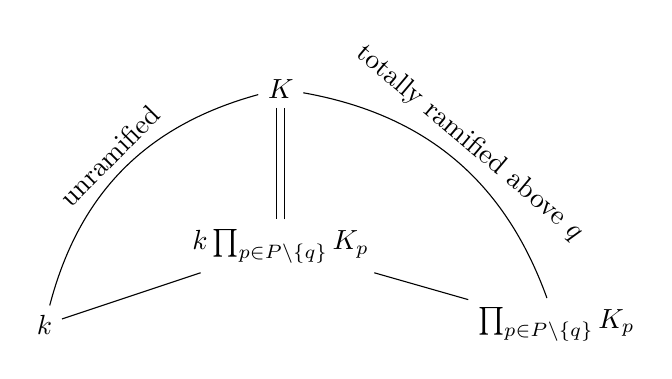
\begin{tikzpicture}
  \node (a) at (0,4)  {$K$};
  \node (b) at (0,2)  {$k\prod_{p\in P\setminus\{q\}}K_p$};
  \node (c) at (-3,1)  {$k$};
  \node (d) at (3.5,1)  {$\prod_{p\in P\setminus\{q\}}K_p$};
  \draw[transform canvas={xshift=-1.5pt}] (a) -- (b);
  \draw[transform canvas={xshift=1.5pt}] (b) -- (a);
  \draw   (b) --  (c)
   (b) -- (d);
  \draw[bend left](c) to node [above , sloped]{\text{unramified}}(a);
  \draw[bend right](d) to node [above , sloped]{\text{totally ramified above $q$}}(a);
\end{tikzpicture}
\end{center}
\end{DESCRIPTION}
\end{proof}

\begin{rem}
Note that for any $p\in P$, the field $K_p$ in the statement of Lemma \ref{genus} is really determined uniquely, because
 by the ramification requirement, it must be a subfield of the cyclotomic field $\Q(\zeta_{p^f})$ for some $f\in\Nbb$, whose absolute Galois group is isomorphic to $(\Z/p^f\Z)^{\times}$, which is cyclic iff $p\geq 3$ or $f\leq 2$, and cyclic groups have at exactly one quotient group of any possible order. The assumption of the cyclicity of all inertia groups in the statement of the lemma is thus not required for $p\geq 3$ or $f\leq 2$, and can be also be removed for the other cases (but then there are three possible choices for $K_2$, so we must slightly change the statement).
\end{rem}

\iffalse
\begin{lemma}\label{comp}
We have $kK_iK_jK_l=K$ and $K_1K_2K_3K_4=K$.
\end{lemma}
\begin{proof}
The extension $K/K_iK_jK_l$ is totally ramified at the prime ideals above $p_h$, so the same must be true for the extension $K/kK_iK_jK_l$. But since the extension $K/k$ is unramified (by the definition of $K$), so is $K/kK_iK_jK_l$. Therefore $[K:kK_iK_jK_l]=1$. The second claim follows from the facts %$\Gal(K_i/\Q)\cong$
$T_i=\Gal(K/K_jK_lK_h)$ and $G=T_1\times T_2\times T_3\times T_4$.
\end{proof}
\begin{center}
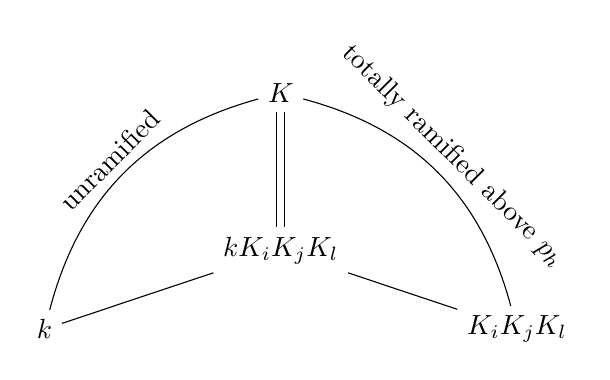
\begin{tikzpicture}
  \node (a) at (0,4)  {$K$};
  \node (b) at (0,2)  {$kK_iK_jK_l$};
  \node (c) at (-3,1)  {$k$};
  \node (d) at (3,1)  {$K_iK_jK_l$};
  \draw[transform canvas={xshift=-1.5pt}] (a) -- (b);
  \draw[transform canvas={xshift=1.5pt}] (b) -- (a);
  \draw   (b) --  (c)
   (b) -- (d);
  \draw[bend left](c) to node [above , sloped]{\text{unramified}}(a);
  \draw[bend right](d) to node [above , sloped]{\text{totally ramified above $p_h$}}(a);
\end{tikzpicture}
\end{center}
\fi


\begin{definition}
Let $G$ be any group. The (integral) \textit{group ring} $\Z[G]$ is the free $\Z$-module with basis $G$, which is made into a ring, extending linearly the group law on $G$.
\end{definition}

\begin{definition}
An element $\alpha$ of a totally real number field $K$ is called totally positive if for any embedding $\sigma: K\to \R$, we have $\sigma(\alpha)>0$.
\end{definition}

\section{The group of circular numbers}
Let $k\neq \Q$ be a real abelian field, $K$ its the genus field in the narrow sense, $P\neq \emptyset$ be the set of ramified primes of $k$ and $K_p$ be the maximal subfield of $K$ ramified only at $p\in P$. Since $\Gal(K/\Q)$ has a natural action on $K$ (given by evaluating an automorphism on an element), this makes $K$ into a $\Z[\Gal(K/\Q)]$-module. 

The following definition is equivalent to Lettl's modification of Sinnott's definition:
\begin{definition}
The group $D(k)$ of circular numbers of $k$ is given as
$$D:=\big\langle \{-1, \eta_I \big\vert \emptyset \subsetneq I \subseteq P \}\big\rangle_{\Z[\Gal(K/\Q)]},$$
where $\langle \dots \rangle_{\Z[\Gal(K/\Q)]}$ means \enquote{generated as a $\Z[\Gal(K/\Q)]$-submodule of $K$} and $$\eta_I=\text{N}_{\Qbb(\zeta_{\text{cond} \left(\prod_{i\in I}K_i\right)})/\left(\prod_{i\in I}K_i)\right)\cap k}\left(1-\zeta_{\text{cond} \left(\prod_{i\in I}K_i\right)}\right),$$ where $\text{N}$ denotes the norm operator and the product of fields denotes their compositum. The subgroup of totally positive elements of $D(k)$ will be denoted by $D^+(k)$.
\end{definition}

\begin{definition}
The group $C(k)$ of circular numbers of $k$ is $E(k)\cap D(k)$, where $E(k)$ is the group of units of the ring of algebraic integers of $k$. The subgroup of totally positive elements of $C(k)$ will be denoted by $C^+(k)$.
\end{definition}

\begin{rem}
All the generators $\eta_I$ of $D$ are totally positive, because they are defined as norms of elements from an imaginary field to a real field. Hence they are images of a product of pairs of complex conjugate automorphisms, and as such they must become positive upon fixing an embedding $\sigma:k\to \R$. On the other hand, $-1$ is not totally positive and its product with any totally positive element is also not totally positive. This shows that $$D^+(k)=\big\langle  \eta_I \big\vert \emptyset \subsetneq I \subseteq P\big\rangle_{\Z[\Gal(K/\Q)]},$$
which is canonically isomorphic to the to torsion-free part of $D(k)$. Since $\Z$ is a principal ideal domain and $D(k)$ is finitely generated, this implies that $D^+(k)$ and consequently also $C^+(k)$ are free $\Z$-modules.
\end{rem}

In \citep{Lettl1990}, it is proven that the previous definition of $C(k)$ gives the same group as Sinnott's original definition in \citep{SinnottAb}. One of the reasons that $C(k)$ is important is the following result, due to Sinnott:
\begin{theorem}\label{finind}
The index $[E(k):C(k)]$ is finite.
\end{theorem}
\begin{proof}
See \citep{SinnottAb}, Theorem 4.1.
\end{proof}

\begin{lemma}\leavevmode \label{units}
\begin{enumerate}%[i)]
\item For $|I|>1$, we have $\eta_I\in E(k)$.
\item For $|I|$, we have $\eta_I\not\in E(k)$, but $\eta_I^{1-\sigma}\in E(k)$ for any $\sigma\in \Gal(K/\Q)$. % in the inertia subgroup of $\Gal(K/\Q)$ corresponding to $p$.
\end{enumerate}
\end{lemma}
\begin{proof}
Since all $\eta_I$ are algebraic integers, it suffices to compute their absolute norm. We have 
\begin{align*}
\N_{\prod_{i\in I}K_i\cap k/\Q}(\eta_I)&=\N_{\Qbb(\zeta_{\text{cond} \left(\prod_{i\in I}K_i\right)})/\Q}
(1-\zeta_{\cond\left(\prod_{i\in I}K_i\right)})\\
&=\begin{cases}
p & \quad \text{ if } \cond\left(\prod_{i\in I}K_i\right) \text{ is a power of a prime } p,\\
1 & \quad \text{ otherwise } \\
\end{cases}
\end{align*}
using the computation in \citep{Sedlacek2015thesis}, page 29. Now, we know that $\Q(\cond\left(\prod_{i\in I}K_i\right))$ is ramified at the same primes as $\prod_{i\in I}K_i$ (this follows from the fact that the intersection of cyclotomic fields is again a cyclotomic field), hence $\N_{\prod_{i\in I}K_i\cap k/\Q}(\eta_I)=1$ iff $|I|>1$. Moreover, for any $I$ and any $\sigma\in \Gal(K/\Q)$, we have $\N_{\prod_{i\in I}K_i\cap k/\Q}(\eta_I)=\N_{\prod_{i\in I}K_i\cap k/\Q}(\sigma(\eta_I))$, hence $\N_{\prod_{i\in I}K_i\cap k/\Q}(\eta_I^{1-\sigma})=1$, which proves the rest of the assertion.
%This follows from \citep{SinnottAb}, Lemma 4.1. %nebo bakalářka?
\end{proof}

\begin{cor}
We have $$C(k)=\big\langle \{ -1, \eta_I \big\vert I \subseteq P,  |I|\geq 2\} \cup \{\eta_I^{1-\sigma} \big\vert |I|=1, \sigma\in \Gal(K/\Q))\}\big\rangle_{\Z[\Gal(K/\Q]}$$
and
$$C^+(k)=\big\langle \{ \eta_I \big\vert I \subseteq P,  |I|\geq 2\} \cup \{\eta_I^{1-\sigma} \big\vert |I|=1, \sigma\in \Gal(K/\Q))\}\big\rangle_{\Z[\Gal(K/\Q]}.$$
\end{cor}

\begin{prop}\label{Drank}
The $\Z$-rank of $D^+(k)$ is $[k:\Q]+|P|-1$ and the $\Z$-rank of $C^+(k)$ is $[k:\Q]-1$.
\end{prop}
\begin{proof}
By Dirichlet's unit theorem, the $\Z$-rank of $E(k)$ is $[k:\Q]-1$, since all the embeddings of $k$ are real. Since the index $[E(k):C(k)]$ is finite by Theorem \ref{finind},  the $\Z$-rank of $C(k)$ must be $[k:\Q]-1$ as well. Since $C^+(k)$ is isomorphic to the torsion-free part of $C(k)$, its $\Z$-rank must also be $[k:\Q]-1$
%Because $C(k)$ is finitely generated, its torsion subgroup is finite, hence the $\Z$-rank of $C^+(k)$, which is isomorphic to the non-torsion part of $C(k)$ by Lemma \ref{torsion}, must also be $[k:\Q]-1$.

Now consider the quotient module $D^+(k)/C^+(k)$. By Lemma \ref{units}, it is generated as a $\Z$-module by the images of $\eta_I$ for $|I|=1$, hence it has exactly $|P|$ generators. Since the absolute norm of $\eta_{\{p\}}$ is a power of $p$%odkaz na bakalářku?
, the elements $\eta_I$ with $|I|=1$ are multiplicatively independent (any nontrivial relation between them would give us a nontrivial multiplicative relation between powers of different primes, which is not possible). Moreover, since the absolute norm of all elements in $C^+$ is $1$, the images of $\eta_I$ remain multiplicatively independent in $D^+(k)/C^+(k)$. Thefore this quotient module has $\Z$-rank $|P|$, which implies that the $\Z$-rank of $D^+$ is $[k:\Q]+|P|-1$ by the first part.
\end{proof}

\section{Notation and assumptions}
In the remainder of the thesis, we will fix $k$ to be a real abelian field with exactly four ramified primes $p_1,p_2,p_3,p_4$ and we will abbreviate $D(k),D^{+}(k),C(k),C^+(k)$ simply as $D,D^{+},C,C^+$. We will alsso use the convention that whenever any of the indices $i,j,l,h$ appear on the same line, they are pairwise distinct and moreover $1\leq i,j,l,h\leq 4$, unless stated otherwise. Finally, for any $n\in \Nbb$, $\zeta_n$ will denote a primitive $n$-th root of unity (WLOG we can take $\zeta_n=e^{2\pi i/n}$). 

\paragraph*{}
Let $K$ be the genus field in the narrow sense of $k$ and let $G:=\Gal(K/\Q)$. Then by Lemma \ref{genus}, we can identify $G$ with the direct product $T_1\times T_2\times T_3\times T_4$, where $T_i$ is the inertia group corresponding the ramified prime $p_i$. Next, we will define:

\begin{itemize}
\item $H:=\Gal(K/k)$, 
\item $m:=|H|,$
\item the canonical projections $\pi_i:G\to T_i$ ,
\item $a_i:=[T_i:\pi_i(H)]$,
\item $r_i:=|H\cap \ker \pi_i|$,
\item $s_{ij}:=|H\cap \ker (\pi_i\pi_j)|$,
\item $n_i:=\frac{m}{r_i}$,
\item $\eta:=\eta_{\{1234\}}$,
\item $K_i$ as the maximal subfield of $K$ ramified only at $p_i$ (so that $$T_i=\Gal(K/K_jK_lK_h)\cong \Gal(K_i/\Q)$$ by Lemma \ref{genus}.)
\end{itemize}

We will assume the following: \label{assum}
\begin{itemize}
%\item $K\neq k$,
\item $H$ is cyclic, generated by $\tau$,
\item each $T_i$ is cyclic, generated by $\sigma_i$.
\end{itemize}
%\begin{rem}
Note that the second assumption isn't very restrictive, as it is automatically true for example if all the ramified primes of $k$ are odd (because $T_i\cong \Gal(K_i/\Q)$ is a quotient of the Galois group $\Gal(\Q(\zeta_{\cond{K_i}})/\Q)\cong (\Z/p_i^e\Z)^{\times}$ for some $e\in\Nbb$).
%\end{rem}

\section{Auxiliary results}
\begin{lemma}\label{tau}
Without loss of generality, we can assume $\tau=\sigma_1^{a_1}\sigma_2^{a_2}\sigma_3^{a_3}\sigma_4^{a_4}$.
\end{lemma}
\begin{proof}
We know that $a_i=[T_i:\pi_i(H)]$, hence
$\pi_i(\tau)$ generates a subgroup of $T_i$ of index $a_i$. The cyclicity of $T_i$ then implies that $\pi_i(\tau)$ must be the $a_i$-th power of some generator of $T_i$, WLOG $\sigma_i$. The statement now follows, because $\tau$ is determined by its four projections.
\end{proof}

%Přidat zvláštní lemma o Galoisových grupách K_iK_jK_l/K_i a podobně kvůli čitelnosti?

\begin{prop}\label{degrees}
We have $$a_i=[k\cap K_i:\Q],$$ $$r_i=[K:kK_i],$$ $$|T_i|=a_in_i,$$ $$s_{ij}=[K:kK_iK_j],$$ $$[K_i:k\cap K_i]=n_i,$$ $$[K_iK_j:k\cap K_iK_j]=\frac{m}{s_{ij}}$$ and $$[K_iK_jK_l:k\cap K_iK_jK_l]=m.$$
\end{prop}
\begin{proof}
Since
\begin{equation*}
\begin{split}
\Gal(K/K_i)&=\Gal(K/K_iK_jK_l\cap K_iK_jK_h\cap K_iK_lK_h)\\
&=\Gal(K/K_iK_jK_l)\cdot \Gal(K/K_iK_jK_h)\cdot \Gal(K/K_iK_lK_h)
= T_jT_lT_h
\end{split}
\end{equation*} 
%$$\Gal(K/K_i)\cong \Gal(K/\Q)/\Gal(K_i/\Q)\cong T_1T_2T_3T_4/T_i\cong T_jT_lT_h$$
 and $\Gal(K/k)=H$, it follows that $\Gal(K/k\cap K_i)= T_jT_lT_h\cdot H$. Now consider the short exact sequence %(clearly $\ker \pi_i=T_jT_lT_h$) 
$$0\to H\cap \ker \pi_i\to H \xrightarrow{\restr{\pi_i}{H}} \pi_i(H)\to 0.$$
It follows that $|\pi_i(H)|=\frac{m}{r_i}=n_i$ and $$\pi_i(H)\cong \frac{H}{H\cap \ker \pi_i}=\frac{H}{H\cap T_jT_lT_h}\cong \frac{T_jT_lT_h\cdot H}{T_jT_lT_h}= \frac{\Gal(K/k\cap K_i)}{\Gal(K/K_i)}\cong \Gal(K_i/k\cap K_i).$$
Therefore 
$$[k\cap K_i:\Q]=\frac{|\Gal(K_i/\Q)|}{|\Gal(K_i/k\cap K_i)|}=\frac{|T_i|}{|\pi_i(H)|}=a_i$$
%$$[k\cap K_i:\Q]=\frac{|T_1T_2T_3T_4|}{|T_jT_lT_h\cdot H|}=\frac{|T_1T_2T_3T_4|\cdot |H\cap T_jT_lT_h|}{|T_jT_lT_h|\cdot |H|}=\frac{|T_i|}{|\pi_i(H)|}=a_i.$$
and
$$[K:kK_i]=\frac{|\Gal(K/k)|}{|\Gal(kK_i/k)|}=\frac{|H|}{|\Gal(K_i/k\cap K_i)|}=\frac{m}{|\pi_i(H)|}=r_i.$$
Putting everything together, we obtain $$|T_i|=[K_i:k\cap K_i]\cdot[k\cap K_i:\Q]=a_i|\pi_i(H)|=a_in_i.$$
Next, we also have 
\begin{equation*}
\begin{split}
\Gal(K/K_iK_j)&=\Gal(K/K_iK_jK_l\cap K_iK_jK_h)\\
&=\Gal(K/K_iK_jK_l)\cdot \Gal(K/K_iK_jK_h)= T_lT_h
\end{split}
\end{equation*} 
%$$\Gal(K/K_iK_j)\cong \Gal(K/\Q)/\Gal(K_iK_j/\Q)\cong T_1T_2T_3T_4/T_iT_j\cong T_lT_h,$$
so that $\Gal(K/k\cap K_iK_j)=T_lT_h\cdot H$. Thus we can consider the short exact sequence 
$$0\to H\cap \ker \pi_i\pi_j\to H \xrightarrow{\restr{\pi_i\pi_j}{H}} \pi_i\pi_j(H)\to 0$$
to conclude that $|\pi_i\pi_j(H)|=\frac{m}{s_{ij}}$ and 
\begin{equation*}
\begin{split}
\pi_i\pi_j(H)&\cong \frac{H}{H\cap \ker \pi_i\pi_j}=\frac{H}{H\cap T_lT_h}\cong \frac{T_lT_h\cdot H}{T_lT_h}\\
&\cong \frac{\Gal(K/k\cap K_iK_j)}{\Gal(K/K_iK_j)}\cong \Gal(K_iK_j/k\cap K_iK_j).
\end{split}
\end{equation*}
Then it follows that 
$$[K:kK_iK_j]=\frac{|\Gal(K/k)|}{|\Gal(kK_iK_j/k)|}=\frac{|H|}{|\Gal(K_iK_j/k\cap K_iK_j)|}=\frac{m}{|\pi_i\pi_j(H)|}=s_{ij}.$$
The last part of the statement is a consequence of Lemma \ref{genus}, since we have $$\Gal(K_iK_jK_l/k\cap K_iK_jK_l)\cong \Gal(kK_iK_jK_l/k)=\Gal(K/k)=H.$$
Finally note that in the same way as above, we could show that $$\pi_i\pi_j\pi_l(H)\cong \frac{H}{H\cap T_h}\cong H$$
(since Lemma \ref{genus} implies that $|H\cap T_h|=1$).
%Finally note that in the same way as above, we could show that $$\pi_i\pi_j\pi_l(H)\cong \Gal(K_iK_jK_l/k\cap K_iK_jK_l).$$
\end{proof}
\begin{center}
\begin{tikzpicture}
  \node (a) at (0,4)  {$K$};
  \node (b) at (0,2)  {$kK_i$};
  \node (c) at (-2,0)  {$k$};
  \node (d) at (2,0)  {$K_i$};
  \node (e) at (0,-2)  {$k\cap K_i$};
  \node (f) at (0,-4)  {$\Q$};
  \draw   (a) -- node [left]{$r_i$} (b) -- node [above left]{$n_i$} (c) -- (e) -- node [below right]{$|\pi_i(H)|$} (d) -- node [above right]{$\frac{|T_j\times T_l\times T_h|}{r_i}$} (b)
  (e) -- node [left]{$a_i$} (f);
\end{tikzpicture}
\qquad
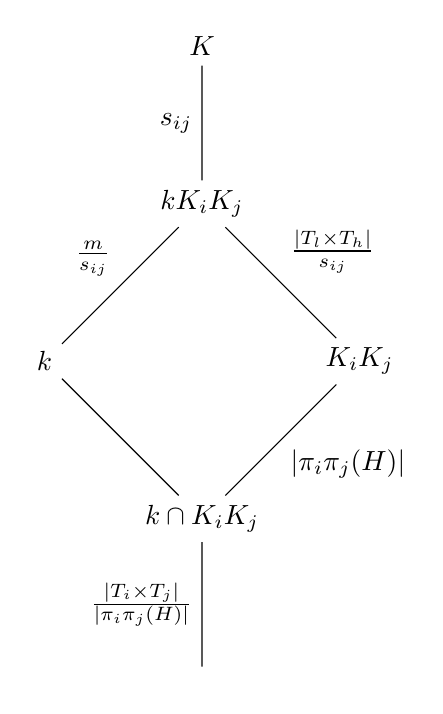
\begin{tikzpicture}
  \node (a) at (0,4)  {$K$};
  \node (b) at (0,2)  {$kK_iK_j$};
  \node (c) at (-2,0)  {$k$};
  \node (d) at (2,0)  {$K_iK_j$};
  \node (e) at (0,-2)  {$k\cap K_iK_j$};
  \node (f) at (0,-4)  {$\Q$};
  \draw   (a) -- node [left]{$s_{ij}$} (b) -- node [above left]{$\frac{m}{s_{ij}}$} (c) -- (e) -- node [below right]{$|\pi_i\pi_j(H)|$} (d) -- node [above right]{$\frac{|T_l\times T_h|}{s_{ij}}$} (b)
  (e) -- node [left]{$\frac{|T_i\times T_j|}{|\pi_i\pi_j(H)|}$} (f);
\end{tikzpicture}
%\vspace{3\baselineskip}
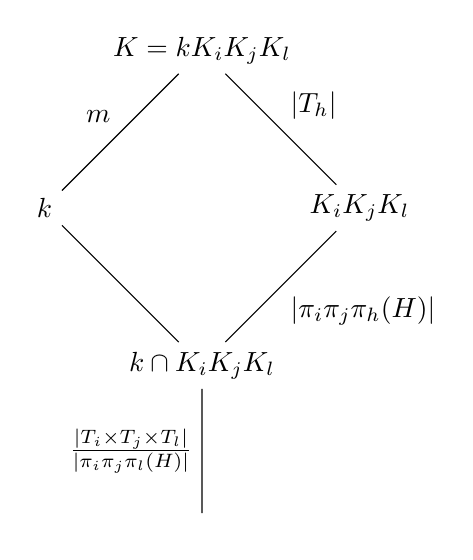
\begin{tikzpicture}
  \node (a) at (0,2)  {$K=kK_iK_jK_l$};
  \node (c) at (-2,0)  {$k$};
  \node (d) at (2,0)  {$K_iK_jK_l$};
  \node (e) at (0,-2)  {$k\cap K_iK_jK_l$};
  \node (f) at (0,-4)  {$\Q$};
  \draw   (a) -- node [above left]{$m$} (c) -- (e) -- node [below right ]{$|\pi_i\pi_j\pi_h(H)|$} (d) -- node [above right]{$|T_h|$} (a)
  (e) -- node [left]{$\frac{|T_i\times T_j\times T_l|}{|\pi_i\pi_j\pi_l(H)|}$} (f);
\end{tikzpicture}
\end{center}

\begin{cor}\label{compcap}
We have $$[k\cap K_iK_j:\Q]=a_ia_j\frac{m}{r_ir_j}s_{ij},$$ $$[k\cap K_iK_jK_l:\Q]=a_ia_ja_l\frac{m^2}{r_ir_jr_l}$$ and $$[k:\Q]=a_1a_2a_3a_4\frac{m^3}{r_1r_2r_3r_4}.$$
\end{cor}
\begin{proof}
This follows from the computations
$$[k\cap K_iK_j:\Q]=\frac{[K_iK_j:\Q]}{[K_iK_j:k\cap K_iK_j]}=\frac{|T_i|\cdot|T_j|}{m/s_{ij}}=a_ia_j\frac{m}{r_ir_j}s_{ij},$$
$$[k\cap K_iK_jK_l:\Q]=\frac{[K_iK_jK_l:\Q]}{[K_iK_jK_l:k\cap K_iK_jK_l]}=\frac{|T_i|\cdot|T_j|\cdot|T_l|}{m}=a_ia_ja_l\frac{m^2}{r_ir_jr_l}$$
and
\begin{equation*}
\begin{split}
[k:\Q]&=\frac{[K:\Q]}{[K:k]}=\frac{|T_1|\cdot|T_2|\cdot|T_3|\cdot|T_4|}{m}=
a_1a_2a_3a_4\frac{m^3}{r_1r_2r_3r_4}.
%[k:\Q]&=[k\cap K_i:\Q]\cdot [k:k\cap K_i]=a_i\cdot [kK_i:K_i]=a_i\frac{[K:K_i]}{[K:kK_i]}\\
%&=a_i\frac{|T_j|\cdot|T_l|\cdot|T_h|}{r_i}=
%a_1a_2a_3a_4\frac{m^3}{r_1r_2r_3r_4}.
\end{split}
\end{equation*}

\end{proof}
\begin{lemma}\label{coprime}
We have 

$$s_{ij}=\gcd(r_i,r_j),$$ $$\gcd(r_i,r_j,r_l)=1,$$ $$\lcm\left(n_i,n_j,n_l\right)=m$$ and $$s_{ij}\frac{m}{r_ir_j}=\gcd(n_i,n_j).$$
\end{lemma}
\begin{proof}
It follows from Proposition \ref{degrees} that $s_{ij}\mid r_i, s_{ij}\mid r_j$ and from its proof that $$|\pi_i(H)|=n_i, \quad |\pi_i\pi_j(H)|=\frac{m}{s_{ij}} \text{ and } |\pi_i\pi_j\pi_l(H)|=m.$$ The cyclicity of $H$ then implies
$$\frac{m}{s_{ij}}=|\pi_i\pi_j(H)|=|\langle\pi_i\pi_j(\tau)\rangle|=|\langle\pi_i(\tau)\pi_j(\tau)\rangle|=\lcm\left(n_i,n_j\right),$$
because $\langle\pi_i(\tau)\rangle=\pi_i(H)$ and any power of the product $\pi_i(\tau)\pi_j(\tau)$ is trivial if and only if the same power of both its factors is (since $G$ is the direct product of the $T_i$'s). 
%the elements $\pi_i(H),\pi_j(H)$ have different non-zero coordinates in $G$.
Now for any common divisor $t$ of $r_i,r_j$, we have $$\frac{m}{s_{ij}}= \lcm\left(n_i,n_j\right)=\lcm\left(\frac{m}{r_i},\frac{m}{r_j}\right) \mid \frac{m}{t},$$ which implies $t\mid s_{ij}$. Hence $s_{ij}=\gcd(r_i,r_j)$.

Similarly, we have
$$m=|\pi_i\pi_j\pi_l(H)|=|\langle\pi_i\pi_j\pi_l(\tau)\rangle|=|\langle\pi_i(\tau)\pi_j(\tau)\pi_l(\tau)\rangle|=\lcm(n_i,n_j,n_l),$$
so if $t$ is any common divisor of $r_i,r_j,r_l$, we have $$m=\lcm(n_i,n_j,n_l)=\lcm\left(\frac{m}{r_i},\frac{m}{r_j},\frac{m}{r_l}\right) \mid \frac{m}{t},$$ which implies $t=1$. This implies both $m=\lcm(n_i,n_j,n_l)$ and $\gcd(r_i,r_j,r_l)=1$ (in fact, these are equivalent).

Finally, using the first result, we have $$s_{ij}\frac{m}{r_ir_j}=\frac{m}{r_ir_j/s_{ij}}=\frac{m}{\lcm(r_i,r_j)},$$ which clearly divides both $\frac{m}{r_i}=n_i$ and $\frac{m}{r_j}=n_j$. Moreover, if $t$ is any common divisor of $n_i=\frac{m}{r_i}$ and $n_j=\frac{m}{r_j}$, then both $r_it$ and $r_jt$ divide $m$, hence $t\cdot\lcm(r_i,r_j)=\lcm(r_it,r_jt)\mid m$. Thus $t\mid \frac{m}{\lcm(r_i,r_j)}$ and we are done.
\end{proof}

\begin{prop}\label{gal}
We have 
\begin{equation*}
\begin{split}
\Gal(k/\Qbb)\cong
 \{\restr{\sigma_1^{x_1}\sigma_2^{x_2}\sigma_3^{x_3}\sigma_4^{x_4}}{k};~ & 0\leq x_1<a_1\frac{m}{r_1}, 0\leq x_2<a_2\frac{m}{r_2s_{34}}, \\ & 0\leq x_3<a_3\frac{m}{r_3r_4}s_{34},0\leq x_4<a_4\},
\end{split}
\end{equation*}
where each automorphism of $k$ determines the quadruple $(x_1,x_2,x_3,x_4)$ uniquely.
\end{prop}
\begin{proof}
First note that by Lemma \ref{coprime}, we have $$a_3\frac{m}{r_3r_4}s_{34}=a_3\gcd(n_3,n_4)\in\Nbb$$ and $$a_2\frac{m}{r_2s_{34}}=a_2\lcm(r_3,r_4)\frac{m}{r_2r_3r_4}\in\Nbb$$ (this follows from $r_i\mid m$ and $\gcd(r_2,r_3,r_4)=1$), so the expressions make sense. By Corollary \ref{compcap}, the set on the right hand side has at most $|\Gal(k/\Qbb)|$ elements. Now let $\rho$ be any automorphism of $k$. If we can show that $\rho$ determines the quadruple $(x_1,x_2,x_3,x_4)$ belonging to the set on the right hand side uniquely, it will follow that the cardinalities agree and we will be done.

\begin{center}
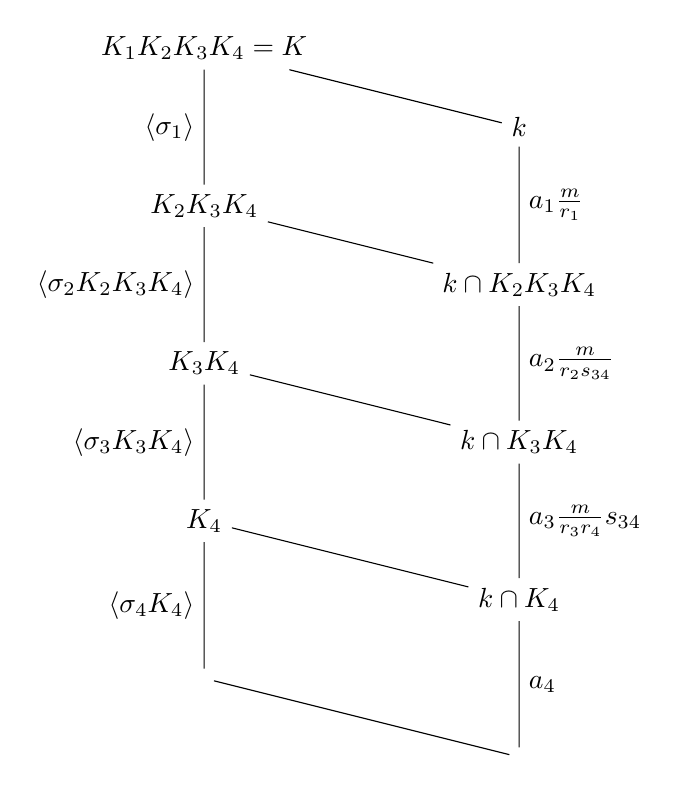
\begin{tikzpicture}
  \node (a) at (0,4)  {$K_1K_2K_3K_4=K$};
  \node (b) at (4,3)  {$k$};
  \node (c) at (0,2)  {$K_2K_3K_4$};
  \node (d) at (4,1)  {$k\cap K_2K_3K_4$};
  \node (e) at (0,0)  {$K_3K_4$};
  \node (f) at (4,-1)  {$k\cap K_3K_4$};
  \node (g) at (0,-2) {$K_4$};
  \node (h) at (4,-3)  {$k\cap K_4$};
  \node (i) at (0,-4) {$\Q$};
  \node (j) at (4,-5)  {$\Q$};
  \draw  (a) -- node [midway,left]{$\langle \sigma_1\rangle$} (c) -- node [midway,left]{$\langle \restr{\sigma_2}{K_2K_3K_4}\rangle$} (e) -- node [midway,left]{$\langle \restr{\sigma_3}{K_3K_4}\rangle$} (g) -- node [midway,left]{$\langle \restr{\sigma_4}{K_4}\rangle$} (i) -- (j) -- node [midway,right]{$a_4$} (h) -- node [midway,right]{$a_3\frac{m}{r_3r_4}s_{34}$} (f) -- node [midway,right]{$a_2\frac{m}{r_2s_{34}}$} (d) -- node [midway,right]{$a_1\frac{m}{r_1}$} (b) -- (a) 
  (c) -- (d)
  (e) -- (f)
  (g) -- (h);
\end{tikzpicture}
\end{center}

Since $\Gal(k\cap K_4/\Q)$ is a cyclic group of order $a_4$ (by Lemma \ref{degrees}) generated by $\restr{\sigma_4}{k\cap K_4}$ (as a quotient of $\Gal(K_4/\Q)=\langle \restr{\sigma_4}{K_4}\rangle$), there must exist a unique $x_4\in \Z$, $0\leq x_4<a_4$ such that $\rho$ and $\sigma_4^{x_4}$ have the same restrictions to $k\cap K_4$. Therefore $\rho\restr{\sigma_4^{-x_4}}{k}\in \Gal(k/k\cap K_4)$. 

Next, $\Gal(k\cap K_3K_4/k\cap K_4)$ is a cyclic group of order $\frac{[k\cap K_3K_4:\Q]}{[k\cap K_4:\Q]}=a_3\frac{m}{r_3r_4}s_{34}$ (by Corollary \ref{compcap}) generated by $\restr{\sigma_3}{k\cap K_3K_4}$ (as it is isomorphic by restriction to $$\Gal((k\cap K_3K_4)K_4 / K_4),$$ which is a quotient of $\Gal(K_3K_4/K_4)=\langle \restr{\sigma_3}{K_3K_4}\rangle$), so there must exist a unique $x_3\in \Z$, $0\leq x_3<a_3\frac{m}{r_3r_4}s_{34}$ such that $\rho \restr{\sigma_4^{-x_4}}{k}$ and $\sigma_3^{x_3}$ have the same restriction to $k\cap K_3K_4$. Therefore $\restr{\rho\sigma_3^{-x_3}\sigma_4^{-x_4}}{k}\in \Gal(k/k\cap K_3K_4)$.

Following the pattern, $\Gal(k\cap K_2K_3K_4/k\cap K_3K_4)$ is a cyclic group of order 
$$\frac{[k\cap K_2K_3K_4:\Q]}{[k\cap K_3K_4:\Q]}=a_2\frac{m}{r_2s_{34}}$$ (by Corollary \ref{compcap}) generated by $\restr{\sigma_2}{k\cap K_2K_3K_4}$ (as it is isomorphic by restriction to $$\Gal((k\cap K_2K_3K_4)K_3K_4 / K_3K_4),$$ which is a quotient of $$\Gal(K_2K_3K_4/K_3K_4)=\langle \restr{\sigma_2}{K_2K_3K_4}\rangle),$$ so there must exist a unique $x_2\in \Z$, $0\leq x_2<a_2\frac{m}{r_2s_{34}}$ such that $\rho\restr{\sigma_3^{-x_3}\sigma_4^{-x_4}}{k}$ and $\sigma_2^{x_2}$ have the same restriction to $k\cap K_2K_3K_4$. Therefore $\restr{\rho\sigma_2^{-x_2}\sigma_3^{-x_3}\sigma_4^{-x_4}}{k}\in \Gal(k/k\cap K_2K_3K_4)$.

Finally, we have $$\Gal(k/k\cap K_2K_3K_4)\cong \Gal(kK_2K_3K_4/K_2K_3K_4)=\Gal(K_1K_2K_3K_4/K_2K_3K_4)=\langle\sigma_1\rangle$$
(using Lemma \ref{genus}), where the isomorphism is given by restriction. Since the order of $\sigma_1$ is $a_1\frac{m}{r_1}$, it follows that there must exist a unique $x_1\in \Z$, $0\leq x_1<a_1\frac{m}{r_1}$ such that $\rho\restr{\sigma_2^{-x_2}\sigma_3^{-x_3}\sigma_4^{-x_4}}{k}$ and $\sigma_1^{x_1}$ have the same restriction to $k$. Thus $\rho=\restr{\sigma_1^{x_1}\sigma_2^{x_2}\sigma_3^{x_3}\sigma_4^{x_4}}{k}$ and the proof is finished.

\end{proof}

%\subsection{Odstavec}

